\documentclass[a4paper,UKenglish]{src/oasics}
\usepackage{microtype}
\usepackage{multirow}
\usepackage{graphics}
\usepackage[normalem]{ulem}
\usepackage{floatrow}

\title{BEST: a Binary Executable Slicing Tool}
\author[1]{Armel Mangean}
\author[2]{Jean-Luc Béchennec}
\author[3]{Mikaël Briday}
\author[3]{Sébastien Faucou}
\affil[1]{École Centrale de Nantes, IRCCyN UMR 6597}
\affil[2]{CNRS, IRCCyN UMR 6597}
\affil[3]{Université de Nantes, IRCCyN UMR 6597}

\Copyright{Armel Mangean, Jean-Luc Béchennec, Mikaël Briday and Sébastien Faucou}
\authorrunning{A. Mangean, J.-L. Béchennec, M. Briday and S. Faucou}
\subjclass{C.3, D2.4, D2.5} % see http://www.acm.org/about/class/ccs98-html
% C.3   Real-Time
% D2.4  Model-Checking
% D2.5  Code Inspection
\keywords{Program Slicing, Binary Code Analysis, WCET Analysis}

\newcommand{\best}{\textsc{Best}}
\newcommand{\h}{\textsc{Harmless}}
\newcommand{\gcc}{\textsc{Gcc}}
\newcommand{\cosmic}{\textsc{Cosmic C}}
\newcommand{\todo}[2]{\textcolor{red}{\bf TODO[#1]\,: #2}}
\newcommand{\JLB}[1]{\textcolor{blue}{\bf JLB\,: #1}}
\usepackage{listings}
\lstnewenvironment{asmlisting}[1][]
  {\lstset{language=C,float=tb,#1}}% \begin{asmlisting}[...]
  {} % \end{asmlisting}

%Editor-only macros:: begin (do not touch as author)%%%%%%%%%%%%%%%%%%%%%%%%%%%%%%%%%%
\EventEditors{John Q. Open and Joan R. Acces}
\EventNoEds{2}
\EventLongTitle{42nd Conference on Very Important Topics (CVIT 2016)}
\EventShortTitle{CVIT 2016}
\EventAcronym{CVIT}
\EventYear{2016}
\EventDate{December 24--27, 2016}
\EventLocation{Little Whinging, United Kingdom}
\EventLogo{}
\SeriesVolume{42}
\ArticleNo{23}
% Editor-only macros::end %%%%%%%%%%%%%%%%%%%%%%%%%%%%%%%%%%%%%%%%%%%%%%%

\begin{document}

  %% \begin{enumerate}
  %%   \item Intro (analyse de wcet par methodes formelles)
  %%   \item related works
  %%   \item contribution
  %%   \item program slicing, overview
  %%   \item l'outil
  %%   \item performance evaluation
  %%   \item conclusion
  %% \end{enumerate}

  \maketitle

  \begin{abstract}
  L'analyse temporelle des systèmes embarqués temps-réel est nécessaire pour
  garantir le respect de l'ensemble de leurs contraintes temporelles. Une telle
  analyse doit déterminer si l'ensemble des exécutions possibles d'un système
  respecte l'ensemble des ses contraintes temporelles. Les différentes analyses
  temporelles existantes s'appuient sur un modèle du programme et un modèle de
  la plateforme matérielle.
  
  Cet article décrit l'implémentation d'un outil de génération de modèles de
  programmes pour l'analyse temporelle par vérification de modèles
  temporisés. Le processus de génération est composé de deux étapes. La première
  réalise une reconstruction du graphe de flot de contrôle du programme à partir
  d'un fichier éxécutable. La seconde procède à une \textit{simplification} du
  graphe de flot de contrôle par \textit{slicing}.
\end{abstract}

  \renewcommand{\baselinestretch}{1.2}
\section{Introduction}
\label{sec:introduction}

  % Nécessité de l'analyse temporelle pour le temps-reél.
  L'analyse temporelle d'un systèmes temps réel doit déterminer si l'ensemble
  des exécutions possibles de ce système respecte les  contraintes temporelles
  exprimées dans sa spécification.  Pour réaliser cette analyse, il faut
  connaître les pires temps d'exécution des tâches qui composent le logiciel du
  système. Ces valeurs sont généralement impossibles à calculer mais il est en
  revanche possible d'en calculer des bornes supérieures.
  Parmi les différentes techniques développées pour cela, nous
  nous intéressons à celles basées sur la théorie de la vérification des
  systèmes temporisés~\cite{DOT10, CB13}. La borne y est
  déterminée en cherchant le plus long chemin dans un modèle obtenu par
  composition d'un modèle du code binaire de la tâche et d'un ensemble de
  modèles des composants de l'architecture matérielle (processeur, pipeline,
  mémoires caches, bus, etc.). Comparées aux autres approches, ces
  techniques permettent une modélisation moins abstraite des comportements
  matériels, ce qui permet d'obtenir des bornes plus
  précises. En revanche, leur application reste limitée par l'explosion
  de la taille l'espace d'état du modèle à analyser~\cite{Wil04}.

  Dans la continuité de~\cite{CB13}, nos travaux visent à
  contribuer au contrôle de la taille de l'espace d'état en réalisant une
  abstraction du code binaire. Cette abstraction consiste à limiter
  l'état du modèle aux valeurs des registres et mots mémoire qui ont un
  impact sur le flot de contrôle. Le calcul de cette abstraction se fait en
  deux étapes. D'abord, le graphe de flots de contrôle du programme est
  reconstruit. Ensuite, ce graphe est analysé \emph{via} un \emph{program slicing}
  pour calculer le sous-ensemble des registres et mots mémoires pertinents.
  Dans la suite, nous nous concentrons sur cette seconde étape.

  %Notre outil est implémenté en C++ et utilise la bibliothèque de manipulation
  %de graphe LEMON \cite{DJK11}.  Les sections \ref{sec:reconstruction} et
  %\ref{sec:slicing} détaillent les aspects théoriques de notre outil. La
  %section \ref{sec:implementation} détaille l'implémentation de notre outil.
  %Enfin, la section \ref{sec:conclusion} présente les perspectives de ce
  %travail.



  %!TEX root = ./main.tex
\section{Related works and contribution}
\label{sec:relatedworks}

  In the context of static WCET analysis, program slicing has been
  explored~\cite{Sandberg2006,Lokuciejewski2009,CB13}. Program slicing is mostly
  used to accelerate the static analysis of flow
  facts~\cite{Sandberg2006,Lokuciejewski2009}. Our goals are different, as well
  as the slicing technique. In contrast to our work, program slicing is applied
  to structured programs at the source code level (or intermediate code
  level~\cite{Sandberg2006}). Our tool works at the binary code level. As a
  positive side effect, it is independent from both the programming language and
  the compiler. To our best knowledge, there is no established tool for slicing
  non-x86 binary code and \best\ aims at filling this gap.

  Our work is the continuation of previous work by Cassez and
  Béchennec~\cite{CB13}. In this work they propose a prototype tool based on the
  classical dataflow equations approach~\cite{Wei81} that computes slices for
  ARM-based binary code. Unlike that, our tool is independent from the target
  instruction set thanks to its interface with the \h\ toolchain. Furthermore,
  our tool is based on a state-of-the-art graph-based approach~\cite{KJL03}. We
  also provide an evaluation focused on the benefits of the program abstraction
  technique.

  Brandner and Jordan~\cite{Brandner2014} propose a graph pruning technique to
  increase the precision of static WCET estimation. Branches of the Control Flow
  Graph (CFG) are pruned based on the criticality of their basic blocks. The
  criticality is defined as the normalized duration of the longest path passing
  through the block~\cite{Brandner2012}. According to the authors this approach
  is akin to ``program slicing in the time domain''. Based on this pruning
  approach, a refinement based WCET calculation meta-algorithm is proposed. We
  do not address a full WCET analysis in this paper. However, their technique
  could be combined with our approach to improve WCET calculation. Such a
  combination should allow to further abstract the program in order to deal with
  state space explosion.







  %!TEX root = ./main.tex
\section{WCET estimation using model-checking}
\label{sec:modelchecking}

  WCET estimation can be reduced to a reachability problem in a network of timed
  automata~\cite{CB13}. The \textsc{Uppaal} tool that supports timed automata
  extended with bounded integer variables is used to build the models, and to
  solve the reachability problem.

  A model of the hardware is built where each architectural feature
  (pipeline(s), cache(s), bus(es), memory, \dots) is modeled by one or more
  timed automata. These automata are synchronized through {\it channels} to
  model the actual hardware behavior. For instance the automaton modeling the
  fetch stage of a pipeline is synchronized with the automaton modeling the
  instruction cache which is synchronized with the automaton modeling the bus
  and so on. The timings of the hardware are modeled by guards and clocks on
  some edges of the automata. A simple model of a memory controller could be the
  timed automaton of Figure~\ref{fig:memaccess}. Notice that this model accounts
  only for the timing.

  \begin{figure}[b]
    \raggedleft
    \floatbox[{\capbeside\thisfloatsetup{capbesideposition={right,center},capbesidewidth=9.3cm}}]{figure}[\FBwidth]
    {\caption{Simple modeling of a memory using \textsc{Uppaal}. In
        the initial state (on the top left) the memory waits for an
        access (MainMemStart synchronization channel). When the access
        is requested, clock $t$ resets and the automaton remains in
        the bottom right state until $t$ reaches the {\scriptsize
          MAINMEMTRANS} value. Then the memory returns to the initial
        state and notifies the end of the memory access (MainMemEnd
        synchronization channel).}\label{fig:memaccess}}
    {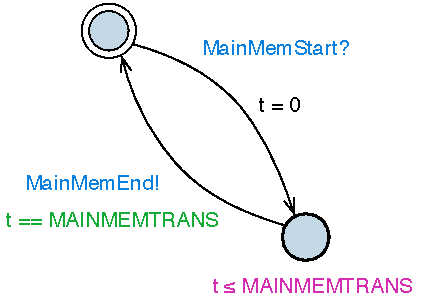
\includegraphics[scale=.6]{fig/automainmem.pdf}}
  \end{figure}

  A model of the program is automatically built from the binary code. In this
  model, each location corresponds to an instruction. An edge leaving a location
  corresponds to the execution of the instruction. For conditional branches, two
  edges leave the location according to the behavior of the branch (taken or not
  taken). Each edge is synchronized with the automaton that models the
  instruction fetch so that it may only be fired if the hardware fetches a new
  instruction. Memory locations are updated according to the semantics of the
  instruction and to its advance in the pipeline. The model of the program has
  an initial state, $I$, that corresponds to the entry point of the program and
  a final state, $F$, that corresponds to the point at which the WCET has to be
  computed.

  At last, a global clock $x$ is used to measure the time. It is initialized at
  0.

  The WCET is then the largest value, $max(x)$, of $x$ when $F$ is
  reached. $max(x)$ can be computed with a model-checker and the following
  reachability property $R(T)$: ``Is $F$ reachable with $x \geq T$ ?''. If
  $R(T)$ is true and $R(T+1)$ is false then $T$ is the WCET of the program.

  This approach is modular since the hardware and software models are built
  separately and the hardware model does not depend on the software to check. No
  assumption is made about the structure of the binary code generated by the
  compiler and the model of the program is built automatically without need for
  annotations

  \paragraph*{Modeling the values stored in memory}

  Data stored in memory and registers -- called a {\it location} in the
  remaining of the paper -- and used by the program can be either included in or
  abstracted away from the model.  Each location included in the model is
  associated with a bounded variable.  When the program accesses a location, the
  timing is computed by the models of the hardware.  If the location is included
  in the model, the associated variable is also read / written.  If the location
  is abstracted away, the data to be written is discarded and any read access
  returns the special value $\bot$.

  On the one hand, every location included in the model adds a dimension to the
  state of the system and thus contributes to the growth of the state space.  On
  the other hand, $\bot$ values can lead the model checker to explore paths that
  are not in the systems when they impact a conditional branch instruction.
  Thus the problem is to automatically compute the minimal set of locations that
  impact on the control flow of the program and that should be included in the
  model.  In this paper, we focus on this problem.


  \section{Réduction d'espace d'état}
\label{sec:slicing}    

    % Program Slicing

    Le \emph{program slicing} \cite{Wei81}, est le calcul d'un sous-ensemble
    d'instructions (\emph{slice}) d'un programme qui affecte les valeurs d'un
    sous-ensemble de ses variables à un certain moment de son exécution. Ce
    sous-ensemble d'instructions est tel qu'il possède un comportement
    équivalent au programme originial vis-à-vis de la valuation du sous-ensemble
    de variables du programme considéré.

    Un \emph{slice} est calculé vis-à-vis d'un critère de \emph{slice}. Celui-ci
    détermine le sous-ensemble des variables du programme ainsi que l'instant
    d'exécution pris en compte. $\mathcal{C}$ est un critère de \emph{slice} tel
    que $\mathcal{C} = \langle l, V \rangle$ avec $l \in \mathcal{L}$ et $V
    \subseteq \mathcal{V}$. Les figures \ref{fig:slice1} et \ref{fig:slice2}
    donne les \emph{slices} du programme \texttt{fibcall-O2.elf} (cf. figure
    \ref{fig:dump}) respectivement pour le critère $\mathcal{C} = \langle 302c,
    \{ r10 \} \rangle$ et le critère $\mathcal{C} = \langle 3030, \{ ctr \}
    \rangle$. $R$ est l'ensemble des variables -- ou registres ici --
    explicitement ou implicitement manipulés qui font l'objet de dépendances de
    données entre les différents blocs de base du CFG. Autrement dit, ce sont
    les variables qui sont à conserver dans l'espace d'état du système pour en
    réaliser une analyse précise et efficace vis-à-vis de leurs valuations
    possibles.

    \begin{figure}[ht]
      \centering
      \begin{subfigure}{.45\textwidth}
        \centering
        \captionsetup{justification=centering}
        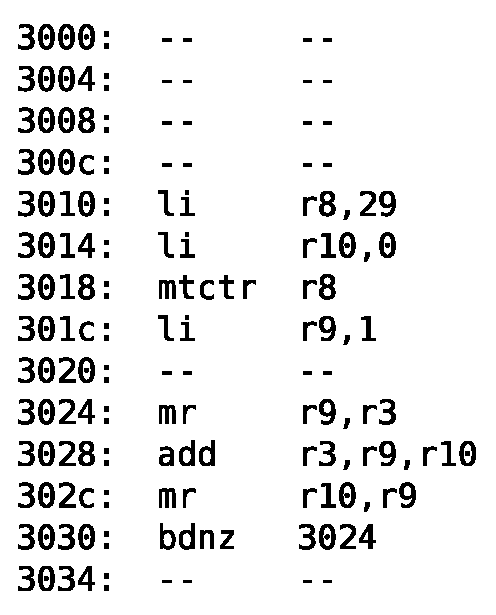
\includegraphics[scale=0.45]{img/slice1.eps}
        \caption{\emph{slice} pour le critère $\mathcal{C} = \langle 302c, \{ r10 \} \rangle$ \\
          $R = \{r3, r8, r9, r10, ctr\}$}
        \label{fig:slice1}
      \end{subfigure}
      \begin{subfigure}{.45\textwidth}
        \centering
        \captionsetup{justification=centering}
        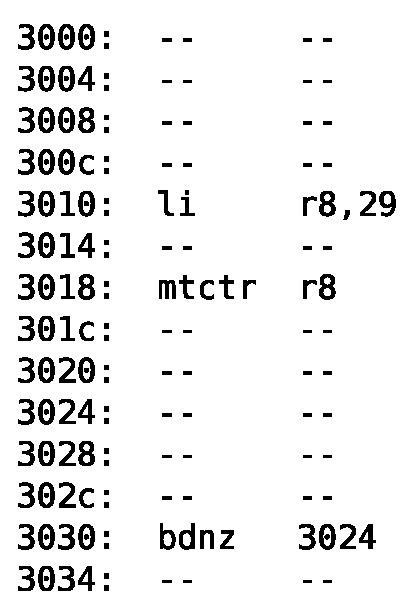
\includegraphics[scale=0.45]{img/slice2.eps}
        \caption{\emph{slice} pour le critère $\mathcal{C} = \langle 3030, \{ ctr \} \rangle$ \\
        $R = \{ctr\}$}
        \label{fig:slice2}
      \end{subfigure}
      \caption{Exemple de \emph{program slicing} d'un fichier binaire exécutable}
    \end{figure}

    %% Quand le \emph{slicing} s'applique à une seule procédure monolithique on
    %% parle de \emph{slicing} intraprocédural. En revanche lorsque le
    %% \emph{slicing} s'applique à un programme entier, au delà des frontières
    %% d'une procédure, on parle de \emph{slicing} interprocedural.
  
    % Intérêt du Program Slicing des CFG pour la vérification de modèle.

    Pour pallier au problème de l'explosion de l'espace d'état inhérent à la
    vérification des modèles il est nécessaire de réduire au maximum la quantité
    d'informations définisant l'état du système. Une utilisation spécifique du
    \emph{program slicing} permet de ne conserver dans l'espace d'état
    du système uniquement les informations définissant l'état des variables --
    registre ou contenu de la pile -- dont la valuation influt directement sur
    le flot de contrôle.

    Il n'est, en effet, pas nécessaire de conserver dans l'espace d'état du
    système les valuations de toutes les variables qui n'agissent pas
    directement sur le flot de contrôle puisqu'elles n'influent pas sur le temps
    d'exécution. Le \emph{slice} donné en figure \ref{fig:slice2} contient
    l'ensemble des instructions du programme \texttt{fibcall-O2.elf} qui agissent
    directement sur le flot de contrôle et manipulent des variables explicitement
    ou implicitement. Il est donc nécessaire de conserver dans l'espace d'état
    du système uniquement la valuation d'un seul registre ($R = \{ ctr$ \}) au
    lieu des 7 registres originaux ($R = \{r1, r3, r8, r9, r10, lr, ctr\}$,
    cf. figure \ref{fig:dump}).
     
    \vspace{1em}
  
    % Program Slicing à base de graphes

    Il existe différentes approches permettant de calculer un \emph{slice}
    \cite{Tip95}.  Cependant, seule la sous catégorie des approches basées sur
    la manipulation de graphes permet de calculer un \emph{slice} pour les
    fichiers binaires exécutables.
    
    Nous nous basons sur une approche permettant de calculer des \emph{slices}
    précis pour les programmes composés de plusieurs procédures (\emph{program
      slicing} interprocédural) \cite{KJL03}.
    
    %% L'algorithme de \emph{slicing} implémenté s'appuie sur la méthode évoquée
    %% ci-après -- cf. \cite{CF97}. Les dépendances de données du programme y sont
    %% représentées par l'arbre post-dominateur et par des chaines de
    %% \emph{use-definition}. Ces chaines relient chaque utilisation d'une
    %% variable aux définitions qui peuvent l'affecter.

    %% Les dépendances de contrôle du programme sont manipulés à travers un graphe
    %% de dépendance de contrôle. Un graphe de dépendance de contrôle est un graphe
    %% où les arcs signifient un lien de dépendance entre la valuation du n{\oe}ud
    %% origine et l'exécution du n{\oe}ud cible.
    

  \section{Implémentation}
\label{sec:implementation}
  
  % Utilisation d'un analyseur sémantique de fichiers exécutables pour la
  % reconstruction de CFG.

  Notre outil manipule des fichiers binaires exécutables compilés pour des
  cibles embarquées à base de microprocesseurs PowerPC. Les informations
  nécessaires à la classification des instructions utiles à la reconstruction
  d'un CFG et au \emph{program slicing} sont issues d'une analyse syntaxique et
  sémantique du fichier binaire exécutable. Cette analyse est produite par un
  outil généré par HARMLESS \cite{KBB12}, un générateur de simulateurs basé sur
  un langage de description de plateformes matérielles.

  \begin{figure}[ht]
    \centering
    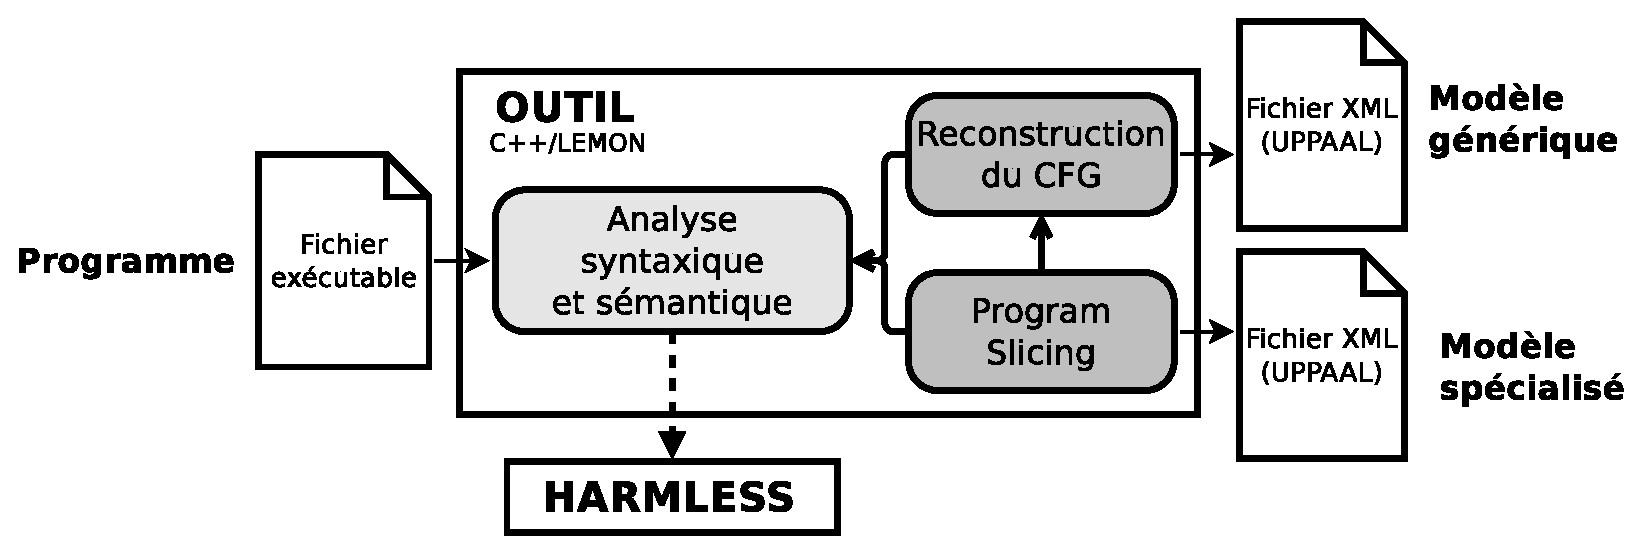
\includegraphics[scale=0.5]{img/archi.eps}
    \caption{Structuration de l'outil}
    \label{fig:implem}
  \end{figure}

  %% Utilisation de la propagation de constante pour rafiner le CFG.
    
  %% Afin de permettre la déterminaison de certaines cibles de saut il est une
  %% nouvelle fois fait usage de l'outil HARMLESS. Celui-ci réalise une
  %% simulation de l'exécution de notre programme sur la plateforme matérielle
  %% considérée. Il est donc possible de procéder à une propagation de constantes
  %% permettant de déterminer des plages de valeurs pour certains registres.

  Notre outil est développé en langage C++, il s'appuie sur une bibliothèque de
  gestion de graphe : LEMON \cite{DJK11}. Les modèles du programme obtenus avant
  ou après \emph{slicing} peuvent être exporter au format Dot, pour être
  visualisés, ainsi que sous forme d'automates temporisés \cite{AD94} au format
  UPPAAL \cite{LPY97}.
  
  Différents tests ont été réalisés à partir des \emph{benchmarks} de Mälardalen
  \cite{GBA10}. Ces \emph{benchmarks} sont utilisés pour évaluer et comparer
  différents outils et méthodes de calcul de pire cas de temps d'exécution.

  %!TEX root = ./main.tex
\section{Experimental results}
\label{sec:results}

  % TODO: (2 pages)
  % - Que veut-on mesurer ?
  % - Définition et justification de notre métrique
  % - Tableaux de résultats et description
  % - Analyse et recul

  We have conducted experiments to measure the reduction of the set of memory
  locations that must be included in the model. Given the current restriction of
  \best{}, we have focused on the registers. To do so, \best\ outputs the
  following information for each program:
  \begin{itemize}
    \item the number of registers used either explicitly or implicitly and the
      number of instructions in the original program ;
    \item the number of registers used either explicitly or implicitly and the
      number of instructions in the sliced program (using the slicing criterion
      defined in Section~\ref{sec:slicing}).
  \end{itemize}
 
  %. For
  %each benchmark we have counted the number $\alpha$ of explicitly and
  %implicitly used registers in the binary executable file. These registers are
  %either from the 32 general purpose registers ($r0$, $r1$, dots, $r32$) or from
  %the 5 dedicated registers ($cr$, $xer$, $lr$, $ctr$, $pc$). Then, we have
  %counted the number $\beta$ of explicitly and implicitly used registers in the
  %slice of the binary executable file according to our specific slicing criteria
  %(see subsection~\ref{subsec:slicing-reduction}). Lastly, we have computed the
  %reduction rate $\gamma = (\alpha - \beta) / \alpha$.

  We used the Mälardalen WCET benchmarks~\cite{Gustafsson:WCET2010:Benchmarks}
  to generate the programs. We had to exclude certain programs to account for the
  current limitation of our tool: program containing floating point arithmetic
  or switch-case statements and recursive programs.

  We used the library generated by the \h\ compiler from a description of a
  PowerPC e200z4 core based on the 32 bits PowerPC instruction set. This
  architecture includes 32 general purpose registers ($r0$, $r1$, \ldots, $r31$)
  and 5 dedicated registers ($cr$, $xer$, $lr$, $ctr$, $pc$). We used two
  different compilers: \gcc\ $5.3.1$ and \cosmic\ $4.3.7$. For a given compiler,
  the generated binary may be very different according to the optimizations. For
  instance without optimization \gcc\ generates code where local variables are
  loaded from and stored to the stack frame each time they are used, whereas in
  higher optimization levels local variables are allocated in registers. Thus we
  created different program versions for each optimization level offered by each
  compiler (4 levels for \gcc\ and 2 levels for \cosmic{}).
  
  All in all, we created 6 versions of each of the 16 Mälardalen benchmarks
  fitting our constraints and we ran \best\ on these 96 programs. Due to space
  limitations the detailed results are provided online\footnote{available at
    \url{https://github.com/TrampolineRTOS/BEST}}. The results are summarized in
  Table~\ref{tab:recap} and~\ref{tab:reginslice}. Table~\ref{tab:recap} gives
  the ratio of registers and instructions in the slice compared to the original
  program. Table~\ref{tab:reginslice} gives the number of registers in the
  slice. It is not meaningful to compare our results with pior work~\cite{CB13}
  because we consider a different instruction set and different compilers (or at
  least compiler version for~\textsc{Gcc}). We do not comment either on the
  execution time of \best\ that were below one second in every case.
  
  \begin{table}
      \centering
      \resizebox{\columnwidth}{!}{%
          \begin{tabular}{|c|c| |c|c|c|c||c|c|c|c|}
   \hline
   \multirow{2}{*}{Compiler} & \multirow{2}*{Optim.} & \multicolumn{4}{c||}{Registers in slice} & \multicolumn{4}{c|}{Instructions in slice} 
   \\\cline{3-10}
    & &  Avg. & Min & Max. & Std. dev. &  Avg. & Min & Max. & Std. dev. 

    \\\hline\hline
    \multirow{4}{*}{\textsc{Gcc}} & \verb|-O0| & 61.8\% & 43.7\%  & 78.9\% & 8.8\% & 21.6\% & 1.7\% & 43.2\% & 8.9\%
    
    \\\cline{2-10}
     & \verb|-O1| & 64.6\% & 19.1\%  & 87.5\% & 13.6\% & 36.7\% & 3.24\% & 67.9\% & 10.2\%
    
    \\\cline{2-10}
     & \verb|-O2| & 64.3\% & 13.3\%  & 92.9\% & 20.3\% & 37.8\% & 2.9\% & 72.5\% & 15.7\%
    
    \\\cline{2-10}
     & \verb|-O3| & 62.8\% & 9\%  & 96.4\% & 21.7\% & 34.7\% & 0.4\% & 72.2\% & 18\%


     \\\hline\hline
     \multirow{2}*{\textsc{Cosmic C}} & \verb|-no| & 40.5\% & 8.6\% & 86.7\% & 16.6\% & 34\% & 1.9\% & 60.2\% & 15.2\% 
    
     \\\cline{2-10}
     & \emph{default} & 37\% & 2.8\% & 66.7\% & 15.8\% & 37\% & 2.8\% & 66.7\% & 15.8\% 
  
     \\\hline
\end{tabular}

%
      }
      \caption{\centering Ratio of registers (resp. instructions) in slice compared to the unsliced program.% \\
      }
      \label{tab:recap}
  \end{table}

  \begin{table}
      \centering
      %\resizebox{.55\columnwidth}{!}{%
      
\begin{tabular}{|c|c|c|c||c|c|}
   \hline
    \multicolumn{4}{|c||}{\textsc{Gcc}} & \multicolumn{2}{c|}{\textsc{Cosmic}} 
    
    \\\hline

    \verb|-O0| & \verb|-O1| &\verb|-O2| &\verb|-O3| & \verb|-no| & \emph{default}

    \\\hline

    8.8 & 13 & 11.8 & 12.1 & 11.9 & 12
  
     \\\hline
\end{tabular}
%
      %}
      \caption{\centering Average number of registers in slice.% \\
      }
      \label{tab:reginslice}
  \end{table}

  
  These results confirm that slicing is an effective abstraction technique for
  our use case.  It allows a significant reduction of the number of variables
  that should be included in the model (reduction of the dimension of the state
  space) as well as the number of instructions the output of which should be
  taken into account (reduction of the number of states to explore).  As
  expected, the best results are obtained for programs with very simple control
  flow, namely \verb|fdct.c| and \verb|jfdctint.c|, whereas the worst results
  are obtained for programs with nested control statements and procedure calls ,
  namely \verb|ndes.c| and \verb|adpcm.c|. However, let us underline that the
  structure of the source code is not always the dominant factor.  For some
  programs, it appears that the compiler (version and/or optimization) has more
  impact on the capacity of the program slicer to abstract the binary. Example
  of such programs are \verb|expint.c| and \verb|fir.c|.

  %% \todo{AM}{Jette un oeil à ces progs. pour voir si tu trouves une
  %% explication}.

   

  
  %\begin{table}
    %\centering
    %\resizebox{.8\columnwidth}{!}{%
    %%!TEX root = ./main.tex
\section{Experimental results}
\label{sec:results}

  % TODO: (2 pages)
  % - Que veut-on mesurer ?
  % - Définition et justification de notre métrique
  % - Tableaux de résultats et description
  % - Analyse et recul

  We have conducted experiments to measure the reduction of the set of memory
  locations that must be included in the model. Given the current restriction of
  \best{}, we have focused on the registers. To do so, \best\ outputs the
  following information for each program:
  \begin{itemize}
    \item the number of registers used either explicitly or implicitly and the
      number of instructions in the original program ;
    \item the number of registers used either explicitly or implicitly and the
      number of instructions in the sliced program (using the slicing criterion
      defined in Section~\ref{sec:slicing}).
  \end{itemize}
 
  %. For
  %each benchmark we have counted the number $\alpha$ of explicitly and
  %implicitly used registers in the binary executable file. These registers are
  %either from the 32 general purpose registers ($r0$, $r1$, dots, $r32$) or from
  %the 5 dedicated registers ($cr$, $xer$, $lr$, $ctr$, $pc$). Then, we have
  %counted the number $\beta$ of explicitly and implicitly used registers in the
  %slice of the binary executable file according to our specific slicing criteria
  %(see subsection~\ref{subsec:slicing-reduction}). Lastly, we have computed the
  %reduction rate $\gamma = (\alpha - \beta) / \alpha$.

  We used the Mälardalen WCET benchmarks~\cite{Gustafsson:WCET2010:Benchmarks}
  to generate the programs. We had to exclude certain programs to account for the
  current limitation of our tool: program containing floating point arithmetic
  or switch-case statements and recursive programs.

  We used the library generated by the \h\ compiler from a description of a
  PowerPC e200z4 core based on the 32 bits PowerPC instruction set. This
  architecture includes 32 general purpose registers ($r0$, $r1$, \ldots, $r31$)
  and 5 dedicated registers ($cr$, $xer$, $lr$, $ctr$, $pc$). We used two
  different compilers: \gcc\ $5.3.1$ and \cosmic\ $4.3.7$. For a given compiler,
  the generated binary may be very different according to the optimizations. For
  instance without optimization \gcc\ generates code where local variables are
  loaded from and stored to the stack frame each time they are used, whereas in
  higher optimization levels local variables are allocated in registers. Thus we
  created different program versions for each optimization level offered by each
  compiler (4 levels for \gcc\ and 2 levels for \cosmic{}).
  
  All in all, we created 6 versions of each of the 16 Mälardalen benchmarks
  fitting our constraints and we ran \best\ on these 96 programs. Due to space
  limitations the detailed results are provided online\footnote{available at
    \url{https://github.com/TrampolineRTOS/BEST}}. The results are summarized in
  Table~\ref{tab:recap} and~\ref{tab:reginslice}. Table~\ref{tab:recap} gives
  the ratio of registers and instructions in the slice compared to the original
  program. Table~\ref{tab:reginslice} gives the number of registers in the
  slice. It is not meaningful to compare our results with pior work~\cite{CB13}
  because we consider a different instruction set and different compilers (or at
  least compiler version for~\textsc{Gcc}). We do not comment either on the
  execution time of \best\ that were below one second in every case.
  
  \begin{table}
      \centering
      \resizebox{\columnwidth}{!}{%
          \begin{tabular}{|c|c| |c|c|c|c||c|c|c|c|}
   \hline
   \multirow{2}{*}{Compiler} & \multirow{2}*{Optim.} & \multicolumn{4}{c||}{Registers in slice} & \multicolumn{4}{c|}{Instructions in slice} 
   \\\cline{3-10}
    & &  Avg. & Min & Max. & Std. dev. &  Avg. & Min & Max. & Std. dev. 

    \\\hline\hline
    \multirow{4}{*}{\textsc{Gcc}} & \verb|-O0| & 61.8\% & 43.7\%  & 78.9\% & 8.8\% & 21.6\% & 1.7\% & 43.2\% & 8.9\%
    
    \\\cline{2-10}
     & \verb|-O1| & 64.6\% & 19.1\%  & 87.5\% & 13.6\% & 36.7\% & 3.24\% & 67.9\% & 10.2\%
    
    \\\cline{2-10}
     & \verb|-O2| & 64.3\% & 13.3\%  & 92.9\% & 20.3\% & 37.8\% & 2.9\% & 72.5\% & 15.7\%
    
    \\\cline{2-10}
     & \verb|-O3| & 62.8\% & 9\%  & 96.4\% & 21.7\% & 34.7\% & 0.4\% & 72.2\% & 18\%


     \\\hline\hline
     \multirow{2}*{\textsc{Cosmic C}} & \verb|-no| & 40.5\% & 8.6\% & 86.7\% & 16.6\% & 34\% & 1.9\% & 60.2\% & 15.2\% 
    
     \\\cline{2-10}
     & \emph{default} & 37\% & 2.8\% & 66.7\% & 15.8\% & 37\% & 2.8\% & 66.7\% & 15.8\% 
  
     \\\hline
\end{tabular}

%
      }
      \caption{\centering Ratio of registers (resp. instructions) in slice compared to the unsliced program.% \\
      }
      \label{tab:recap}
  \end{table}

  \begin{table}
      \centering
      %\resizebox{.55\columnwidth}{!}{%
      
\begin{tabular}{|c|c|c|c||c|c|}
   \hline
    \multicolumn{4}{|c||}{\textsc{Gcc}} & \multicolumn{2}{c|}{\textsc{Cosmic}} 
    
    \\\hline

    \verb|-O0| & \verb|-O1| &\verb|-O2| &\verb|-O3| & \verb|-no| & \emph{default}

    \\\hline

    8.8 & 13 & 11.8 & 12.1 & 11.9 & 12
  
     \\\hline
\end{tabular}
%
      %}
      \caption{\centering Average number of registers in slice.% \\
      }
      \label{tab:reginslice}
  \end{table}

  
  These results confirm that slicing is an effective abstraction technique for
  our use case.  It allows a significant reduction of the number of variables
  that should be included in the model (reduction of the dimension of the state
  space) as well as the number of instructions the output of which should be
  taken into account (reduction of the number of states to explore).  As
  expected, the best results are obtained for programs with very simple control
  flow, namely \verb|fdct.c| and \verb|jfdctint.c|, whereas the worst results
  are obtained for programs with nested control statements and procedure calls ,
  namely \verb|ndes.c| and \verb|adpcm.c|. However, let us underline that the
  structure of the source code is not always the dominant factor.  For some
  programs, it appears that the compiler (version and/or optimization) has more
  impact on the capacity of the program slicer to abstract the binary. Example
  of such programs are \verb|expint.c| and \verb|fir.c|.

  %% \todo{AM}{Jette un oeil à ces progs. pour voir si tu trouves une
  %% explication}.

   

  
  %\begin{table}
    %\centering
    %\resizebox{.8\columnwidth}{!}{%
    %%!TEX root = ./main.tex
\section{Experimental results}
\label{sec:results}

  % TODO: (2 pages)
  % - Que veut-on mesurer ?
  % - Définition et justification de notre métrique
  % - Tableaux de résultats et description
  % - Analyse et recul

  We have conducted experiments to measure the reduction of the set of memory
  locations that must be included in the model. Given the current restriction of
  \best{}, we have focused on the registers. To do so, \best\ outputs the
  following information for each program:
  \begin{itemize}
    \item the number of registers used either explicitly or implicitly and the
      number of instructions in the original program ;
    \item the number of registers used either explicitly or implicitly and the
      number of instructions in the sliced program (using the slicing criterion
      defined in Section~\ref{sec:slicing}).
  \end{itemize}
 
  %. For
  %each benchmark we have counted the number $\alpha$ of explicitly and
  %implicitly used registers in the binary executable file. These registers are
  %either from the 32 general purpose registers ($r0$, $r1$, dots, $r32$) or from
  %the 5 dedicated registers ($cr$, $xer$, $lr$, $ctr$, $pc$). Then, we have
  %counted the number $\beta$ of explicitly and implicitly used registers in the
  %slice of the binary executable file according to our specific slicing criteria
  %(see subsection~\ref{subsec:slicing-reduction}). Lastly, we have computed the
  %reduction rate $\gamma = (\alpha - \beta) / \alpha$.

  We used the Mälardalen WCET benchmarks~\cite{Gustafsson:WCET2010:Benchmarks}
  to generate the programs. We had to exclude certain programs to account for the
  current limitation of our tool: program containing floating point arithmetic
  or switch-case statements and recursive programs.

  We used the library generated by the \h\ compiler from a description of a
  PowerPC e200z4 core based on the 32 bits PowerPC instruction set. This
  architecture includes 32 general purpose registers ($r0$, $r1$, \ldots, $r31$)
  and 5 dedicated registers ($cr$, $xer$, $lr$, $ctr$, $pc$). We used two
  different compilers: \gcc\ $5.3.1$ and \cosmic\ $4.3.7$. For a given compiler,
  the generated binary may be very different according to the optimizations. For
  instance without optimization \gcc\ generates code where local variables are
  loaded from and stored to the stack frame each time they are used, whereas in
  higher optimization levels local variables are allocated in registers. Thus we
  created different program versions for each optimization level offered by each
  compiler (4 levels for \gcc\ and 2 levels for \cosmic{}).
  
  All in all, we created 6 versions of each of the 16 Mälardalen benchmarks
  fitting our constraints and we ran \best\ on these 96 programs. Due to space
  limitations the detailed results are provided online\footnote{available at
    \url{https://github.com/TrampolineRTOS/BEST}}. The results are summarized in
  Table~\ref{tab:recap} and~\ref{tab:reginslice}. Table~\ref{tab:recap} gives
  the ratio of registers and instructions in the slice compared to the original
  program. Table~\ref{tab:reginslice} gives the number of registers in the
  slice. It is not meaningful to compare our results with pior work~\cite{CB13}
  because we consider a different instruction set and different compilers (or at
  least compiler version for~\textsc{Gcc}). We do not comment either on the
  execution time of \best\ that were below one second in every case.
  
  \begin{table}
      \centering
      \resizebox{\columnwidth}{!}{%
          \input{fig/recap}%
      }
      \caption{\centering Ratio of registers (resp. instructions) in slice compared to the unsliced program.% \\
      }
      \label{tab:recap}
  \end{table}

  \begin{table}
      \centering
      %\resizebox{.55\columnwidth}{!}{%
      \input{fig/reginslice}%
      %}
      \caption{\centering Average number of registers in slice.% \\
      }
      \label{tab:reginslice}
  \end{table}

  
  These results confirm that slicing is an effective abstraction technique for
  our use case.  It allows a significant reduction of the number of variables
  that should be included in the model (reduction of the dimension of the state
  space) as well as the number of instructions the output of which should be
  taken into account (reduction of the number of states to explore).  As
  expected, the best results are obtained for programs with very simple control
  flow, namely \verb|fdct.c| and \verb|jfdctint.c|, whereas the worst results
  are obtained for programs with nested control statements and procedure calls ,
  namely \verb|ndes.c| and \verb|adpcm.c|. However, let us underline that the
  structure of the source code is not always the dominant factor.  For some
  programs, it appears that the compiler (version and/or optimization) has more
  impact on the capacity of the program slicer to abstract the binary. Example
  of such programs are \verb|expint.c| and \verb|fir.c|.

  %% \todo{AM}{Jette un oeil à ces progs. pour voir si tu trouves une
  %% explication}.

   

  
  %\begin{table}
    %\centering
    %\resizebox{.8\columnwidth}{!}{%
    %\input{fig/results}%
    %}
    %\caption{\centering Results for Mälardalen benchmark. \\
      %Results in each column are expressed as ``-$\gamma$\%~($\alpha$)''% where \\
%%      $\alpha$ is the number of explicitly and implicitly used registers in the original program ;\\
%%      $\beta$ is the number of explicitly and implicitly used registers in the slice ; \\
%%      $\gamma = (\alpha - \beta) / \alpha \times 100$, the gain in percentage.
      %\\\todo{AM}{Réexporter les données}}
    %\label{tab:results}
  %\end{table}

  
  %Overall, the average reduction is $41\%$ with a standard deviation of $24$.
  %This result \todo{AM}{Comparaison avec ACSD 13 ?}
  %It confirms the interest of the approach.
  %The average reduction is $35\%$ for \gcc\ and $55\%$ for \cosmic{}.
  %The reason is that \cosmic\ uses extensively the general purpose registers:
  %the mean value of $\alpha$ is $32$ in the case of \cosmic\ and $20$ for
  %\gcc\ ($14$ for level \texttt{O0}).
  
  %% It is thus expected that the development of the stack frame analysis will
  %% improve the results in the case of \gcc{}. \todo{AM}{Est-ce certain ?
  %% d'après tes notes, il y a moins de load /store dans gcc optim quand dans
  %% cosmic, néanmoins il y a plus de registre utilisés dans cosmic : il faut
  %% creuser cela}.

  %The worst results are obtained with \verb|ndes.c| compiled with
  %\gcc\ (\verb|-O3|) and \verb|adpcm.c| compiled with \gcc\ (\verb|-O2|). While,
  %the binaries are constituted respectively of 886 and 1094 instructions, the
  %slices are constituted of 522 and 421 instructions, i.e. 62\% and 38\% of the
  %instructions of the original program. \verb|ndes.c| and \verb|adpcm.c| do
  %extensive use of nested control statements (if-then-else statements, for-loop
  %and while-loops) and extensive use of calls to the same small procedures.

  %The best results are obtained with \verb|fdct.c| and and \verb|jfdctint.c|
  %both compiled with \cosmic\. While, the binaries are constituted respectively
  %of 218 and 205 instructions, the slices are constituted of 6 and 9
  %instructions, i.e. 3\% and 4\% of the instructions of the original program.
  %\verb|fdct.c| and \verb|jfdctint.c| are two implementations of the same
  %algorithm. They are made of only two not-nested for-loops with extensive
  %sequential computation in both loops and no procedure call.
  
  %\todo{AM}{On se pose la question de la dépendance des résultats au programme. Pour visualiser cela simplement, on pourrait tracer la courbe de gamma en fonction du programme par compilateur (dans le papier) et par niveau d'optimisation et commenter (sur le site web uniquement).}
  

  %Not optimized binaries produced with \gcc\ does extensive use of the stack
  %with a mean of 174 loads or stores per binary. Lowering the number of memory
  %access is one of the major optimization introduced with the first optimization
  %level on \gcc\ (\verb|-O1|) with a mean of 56 loads or stores per binary.
  %Whereas, not optimized binaries produces with \cosmic\ (\verb|-no|) don't do
  %such an extensive use of the stack with a mean of 89 loads or stores per
  %binary. Lowering the number of memory access is not a major optimization with
  %the default and only optimization level on \cosmic\ with a mean of 79 loads or
  %stores per binary.

  %However, the \cosmic\ compiler does an extensive use of the general purpose
  %registers. Indeed, the mean value of $\alpha$ on \cosmic\ is 32 for not optimized
  %binaries and 32 for the default optimization level while the mean value of
  %$\alpha$ for \gcc\ is 14 for not optimized binaries and respectively 20, 18
  %and 20 for the first, second and third optimization level.

  %In fact, unoptimized binaries produced with \cosmic\ are pretty similar to
  %binaries produced by \gcc\ with the optimization level \verb|-O1|.
  %optimizations techniques embedded in the \cosmic\ compiler consist mainly of
  %instruction number reduction through constant propagation techniques. CFG for
  %two binaries from the same source file compiled with different optimization
  %levels with \cosmic\ are mostly identical while they are pretty different
  %while compiled with two different optimization levels.

  %% Pourquoi les résultats sont plutôt interessant :
  
  %\todo{}{je n'ai pas de recul/je ne maitrise pas ce que je dis}\\
  %\todo{JLB}{Clairement c'est faux :-) on ne peut pas dire ça}
  %Embedded code are, for a large part, made of regulation algebra handling
  %vectors and matrices. In this kind of programs most of the computations does
  %not affect the flow of control of the program. So, considering this kind of
  %programs we can state that our approach has a good potential to yield
  %significant state-pace reductions.

  %However, when it comes to slicing programs like services form a real-time
  %operating system, the computations does strongly affect the flow of control of
  %the program and so the gain may be really low.

%
    %}
    %\caption{\centering Results for Mälardalen benchmark. \\
      %Results in each column are expressed as ``-$\gamma$\%~($\alpha$)''% where \\
%%      $\alpha$ is the number of explicitly and implicitly used registers in the original program ;\\
%%      $\beta$ is the number of explicitly and implicitly used registers in the slice ; \\
%%      $\gamma = (\alpha - \beta) / \alpha \times 100$, the gain in percentage.
      %\\\todo{AM}{Réexporter les données}}
    %\label{tab:results}
  %\end{table}

  
  %Overall, the average reduction is $41\%$ with a standard deviation of $24$.
  %This result \todo{AM}{Comparaison avec ACSD 13 ?}
  %It confirms the interest of the approach.
  %The average reduction is $35\%$ for \gcc\ and $55\%$ for \cosmic{}.
  %The reason is that \cosmic\ uses extensively the general purpose registers:
  %the mean value of $\alpha$ is $32$ in the case of \cosmic\ and $20$ for
  %\gcc\ ($14$ for level \texttt{O0}).
  
  %% It is thus expected that the development of the stack frame analysis will
  %% improve the results in the case of \gcc{}. \todo{AM}{Est-ce certain ?
  %% d'après tes notes, il y a moins de load /store dans gcc optim quand dans
  %% cosmic, néanmoins il y a plus de registre utilisés dans cosmic : il faut
  %% creuser cela}.

  %The worst results are obtained with \verb|ndes.c| compiled with
  %\gcc\ (\verb|-O3|) and \verb|adpcm.c| compiled with \gcc\ (\verb|-O2|). While,
  %the binaries are constituted respectively of 886 and 1094 instructions, the
  %slices are constituted of 522 and 421 instructions, i.e. 62\% and 38\% of the
  %instructions of the original program. \verb|ndes.c| and \verb|adpcm.c| do
  %extensive use of nested control statements (if-then-else statements, for-loop
  %and while-loops) and extensive use of calls to the same small procedures.

  %The best results are obtained with \verb|fdct.c| and and \verb|jfdctint.c|
  %both compiled with \cosmic\. While, the binaries are constituted respectively
  %of 218 and 205 instructions, the slices are constituted of 6 and 9
  %instructions, i.e. 3\% and 4\% of the instructions of the original program.
  %\verb|fdct.c| and \verb|jfdctint.c| are two implementations of the same
  %algorithm. They are made of only two not-nested for-loops with extensive
  %sequential computation in both loops and no procedure call.
  
  %\todo{AM}{On se pose la question de la dépendance des résultats au programme. Pour visualiser cela simplement, on pourrait tracer la courbe de gamma en fonction du programme par compilateur (dans le papier) et par niveau d'optimisation et commenter (sur le site web uniquement).}
  

  %Not optimized binaries produced with \gcc\ does extensive use of the stack
  %with a mean of 174 loads or stores per binary. Lowering the number of memory
  %access is one of the major optimization introduced with the first optimization
  %level on \gcc\ (\verb|-O1|) with a mean of 56 loads or stores per binary.
  %Whereas, not optimized binaries produces with \cosmic\ (\verb|-no|) don't do
  %such an extensive use of the stack with a mean of 89 loads or stores per
  %binary. Lowering the number of memory access is not a major optimization with
  %the default and only optimization level on \cosmic\ with a mean of 79 loads or
  %stores per binary.

  %However, the \cosmic\ compiler does an extensive use of the general purpose
  %registers. Indeed, the mean value of $\alpha$ on \cosmic\ is 32 for not optimized
  %binaries and 32 for the default optimization level while the mean value of
  %$\alpha$ for \gcc\ is 14 for not optimized binaries and respectively 20, 18
  %and 20 for the first, second and third optimization level.

  %In fact, unoptimized binaries produced with \cosmic\ are pretty similar to
  %binaries produced by \gcc\ with the optimization level \verb|-O1|.
  %optimizations techniques embedded in the \cosmic\ compiler consist mainly of
  %instruction number reduction through constant propagation techniques. CFG for
  %two binaries from the same source file compiled with different optimization
  %levels with \cosmic\ are mostly identical while they are pretty different
  %while compiled with two different optimization levels.

  %% Pourquoi les résultats sont plutôt interessant :
  
  %\todo{}{je n'ai pas de recul/je ne maitrise pas ce que je dis}\\
  %\todo{JLB}{Clairement c'est faux :-) on ne peut pas dire ça}
  %Embedded code are, for a large part, made of regulation algebra handling
  %vectors and matrices. In this kind of programs most of the computations does
  %not affect the flow of control of the program. So, considering this kind of
  %programs we can state that our approach has a good potential to yield
  %significant state-pace reductions.

  %However, when it comes to slicing programs like services form a real-time
  %operating system, the computations does strongly affect the flow of control of
  %the program and so the gain may be really low.

%
    %}
    %\caption{\centering Results for Mälardalen benchmark. \\
      %Results in each column are expressed as ``-$\gamma$\%~($\alpha$)''% where \\
%%      $\alpha$ is the number of explicitly and implicitly used registers in the original program ;\\
%%      $\beta$ is the number of explicitly and implicitly used registers in the slice ; \\
%%      $\gamma = (\alpha - \beta) / \alpha \times 100$, the gain in percentage.
      %\\\todo{AM}{Réexporter les données}}
    %\label{tab:results}
  %\end{table}

  
  %Overall, the average reduction is $41\%$ with a standard deviation of $24$.
  %This result \todo{AM}{Comparaison avec ACSD 13 ?}
  %It confirms the interest of the approach.
  %The average reduction is $35\%$ for \gcc\ and $55\%$ for \cosmic{}.
  %The reason is that \cosmic\ uses extensively the general purpose registers:
  %the mean value of $\alpha$ is $32$ in the case of \cosmic\ and $20$ for
  %\gcc\ ($14$ for level \texttt{O0}).
  
  %% It is thus expected that the development of the stack frame analysis will
  %% improve the results in the case of \gcc{}. \todo{AM}{Est-ce certain ?
  %% d'après tes notes, il y a moins de load /store dans gcc optim quand dans
  %% cosmic, néanmoins il y a plus de registre utilisés dans cosmic : il faut
  %% creuser cela}.

  %The worst results are obtained with \verb|ndes.c| compiled with
  %\gcc\ (\verb|-O3|) and \verb|adpcm.c| compiled with \gcc\ (\verb|-O2|). While,
  %the binaries are constituted respectively of 886 and 1094 instructions, the
  %slices are constituted of 522 and 421 instructions, i.e. 62\% and 38\% of the
  %instructions of the original program. \verb|ndes.c| and \verb|adpcm.c| do
  %extensive use of nested control statements (if-then-else statements, for-loop
  %and while-loops) and extensive use of calls to the same small procedures.

  %The best results are obtained with \verb|fdct.c| and and \verb|jfdctint.c|
  %both compiled with \cosmic\. While, the binaries are constituted respectively
  %of 218 and 205 instructions, the slices are constituted of 6 and 9
  %instructions, i.e. 3\% and 4\% of the instructions of the original program.
  %\verb|fdct.c| and \verb|jfdctint.c| are two implementations of the same
  %algorithm. They are made of only two not-nested for-loops with extensive
  %sequential computation in both loops and no procedure call.
  
  %\todo{AM}{On se pose la question de la dépendance des résultats au programme. Pour visualiser cela simplement, on pourrait tracer la courbe de gamma en fonction du programme par compilateur (dans le papier) et par niveau d'optimisation et commenter (sur le site web uniquement).}
  

  %Not optimized binaries produced with \gcc\ does extensive use of the stack
  %with a mean of 174 loads or stores per binary. Lowering the number of memory
  %access is one of the major optimization introduced with the first optimization
  %level on \gcc\ (\verb|-O1|) with a mean of 56 loads or stores per binary.
  %Whereas, not optimized binaries produces with \cosmic\ (\verb|-no|) don't do
  %such an extensive use of the stack with a mean of 89 loads or stores per
  %binary. Lowering the number of memory access is not a major optimization with
  %the default and only optimization level on \cosmic\ with a mean of 79 loads or
  %stores per binary.

  %However, the \cosmic\ compiler does an extensive use of the general purpose
  %registers. Indeed, the mean value of $\alpha$ on \cosmic\ is 32 for not optimized
  %binaries and 32 for the default optimization level while the mean value of
  %$\alpha$ for \gcc\ is 14 for not optimized binaries and respectively 20, 18
  %and 20 for the first, second and third optimization level.

  %In fact, unoptimized binaries produced with \cosmic\ are pretty similar to
  %binaries produced by \gcc\ with the optimization level \verb|-O1|.
  %optimizations techniques embedded in the \cosmic\ compiler consist mainly of
  %instruction number reduction through constant propagation techniques. CFG for
  %two binaries from the same source file compiled with different optimization
  %levels with \cosmic\ are mostly identical while they are pretty different
  %while compiled with two different optimization levels.

  %% Pourquoi les résultats sont plutôt interessant :
  
  %\todo{}{je n'ai pas de recul/je ne maitrise pas ce que je dis}\\
  %\todo{JLB}{Clairement c'est faux :-) on ne peut pas dire ça}
  %Embedded code are, for a large part, made of regulation algebra handling
  %vectors and matrices. In this kind of programs most of the computations does
  %not affect the flow of control of the program. So, considering this kind of
  %programs we can state that our approach has a good potential to yield
  %significant state-pace reductions.

  %However, when it comes to slicing programs like services form a real-time
  %operating system, the computations does strongly affect the flow of control of
  %the program and so the gain may be really low.


  \section{Conclusion}
\label{sec:conclusion}

  % Résumé.

  Cet article décrit le fonctionnement d'un outil de génération de modèles de
  programmes pour l'analyse temporelle des systèmes embarqués temps-réel par
  vérification de modèles temporisés. Les modèles produits sous forme
  d'automates finis sont générés à partir de fichiers exécutables suivant une
  approche de reconstruction de CFG à base de graphes. Ces modèles sont délestés
  d'un certain nombre d'informations qui ne sont pas nécessaires à l'analyse
  temporelle afin de contenir la taille de l'espace d'état qu'ils engendrent.

  % Perspectives associées.

  Les microprocesseurs multi-c{\oe}urs sont de plus en plus employés dans
  l'embarqué temps-réel à des fins de performances et de baisse de consommation
  d'énergie. La réalisation de cet outil fait partie d'un travail de
  développement d'une approche d'analyse temporelle adaptée à ces plateformes
  matérielles.


  
  \appendix
  \bibliographystyle{plain}
  \bibliography{src/refs}

\end{document}
